
\section{Examples}

The previous sections dealt with the main software architecture and program utilities of the UCVM framework. Here we present a few practical examples that demonstrate how to retrieve and plot data from CVMs registered in the framework. Space limitations, however, prevent us from providing examples for all utilities here. The reader should refer to the General User Guide (see Table \ref{tab:manuals}) for additional examples and details, which also includes examples of how to use the UCVM API in C and Fortran codes.

\subsection{Querying Velocity Models}

Querying velocity models is the most basic functionality provided by UCVM. From a terminal, this can be done simply by invoking the command-line tool \texttt{ucvm\_query} as follows.

\begin{lstlisting}[
	frame=none,
	basewidth={0.45em,0.4em},
	basicstyle=\ttfamily\footnotesize,breaklines=true,
	linewidth=0.98\columnwidth,xleftmargin=0.065\columnwidth,
	numbers=left,numberblanklines=true,numberstyle=\scriptsize\color{mylistingnclr},style=optional]
> ./ucvm_query -f $UCVM_DIR/conf/ucvm.conf -m cvms @< [input]@
\end{lstlisting}

\noindent
Here, \texttt{ucvm.conf} is a configuration file which is created at installation time and contains information about the models available in the framework as installed; the flag ``\texttt{-f}'' indicates the location of this configuration file; and the flag ``\texttt{-m}'' preceeds the label of the model from which properties are to be retrieved. The input, which may be optionally given in a file, are the longitude, latitude, and depth of the queried point. Similarly, one can also query a model for the depth of a threshold velocity using the \texttt{basin\_query} command.

\begin{lstlisting}[
	frame=none,
	basewidth={0.45em,0.4em},
	basicstyle=\ttfamily\footnotesize,breaklines=true,
	linewidth=0.98\columnwidth,xleftmargin=0.065\columnwidth,
	numbers=left,numberblanklines=true,numberstyle=\scriptsize\color{mylistingnclr}]
> ./basin_query $UCVM_DIR/conf/ucvm.conf -m cvms -v 2500
\end{lstlisting}

\noindent
In this case, the configuration file parameter requires no flag, and the flag ``\texttt{-v}'' indicates the threshold velocity.

\subsection{Creating Structured and Semi-Unstructured Meshes}

As described before, for creating materialized models int eh form of regular grids or semi-unstructured meshes, UCVM users can use the single-core programs \texttt{ucvm2mesh} and \texttt{ucvm2etree}. These two utilities are invoked similarly by typing:

\begin{lstlisting}[
	frame=none,
	basewidth={0.45em,0.4em},
	basicstyle=\ttfamily\footnotesize,breaklines=true,
	linewidth=0.98\columnwidth,xleftmargin=0.065\columnwidth,
	numbers=left,numberblanklines=true,numberstyle=\scriptsize\color{mylistingnclr}]
> ./ucvm2mesh -f ./ucvm2mesh.conf
\end{lstlisting}

\noindent
and

\begin{lstlisting}[
	frame=none,
	basewidth={0.45em,0.4em},
	basicstyle=\ttfamily\footnotesize,breaklines=true,
	linewidth=0.98\columnwidth,xleftmargin=0.065\columnwidth,
	numbers=left,numberblanklines=true,numberstyle=\scriptsize\color{mylistingnclr}]
> ./ucvm2etree -f ./ucvm2etree.conf
\end{lstlisting}

\noindent
Here, the \texttt{ucvm2mesh.conf} and \texttt{ucvm2etree.conf} are configuration files that specify the model(s) to be queried, the coordinates and dimensions of the regional domain to be meshed, and the projection to be used, as well as the discretization parameters (e.g., gridding size). Paths to the output binary file or etree database are also given in these configuration files.

%\subsection{The \textup{\texttt{ucvm2mesh}} command}
%
%This command generates a mesh or grid in either IJK-12, IJK-20, IJK-32, or SORD formats. The formats IJK-12, IJK-20, IJK-32, for instance, are used in discrete finite difference models for wave propagation simulations by the code \textcolor{red}{AWP-ODC (?) \citep{Cui_2010_Proc}}. SORD, on the other hand, is a format designed to interface with a finite element code used to simulate dynamic rupture processes (also called SORD) \citep{Ely_2009_GJI}. The \texttt{ucvm2mesh} takes as input a configuration file that is passed on as an argument using the flag ``\texttt{-f}''. This file specifies the model to be used, the region size, and the resolution of the mesh or grid. The following example shows how to execute this command.
%
%\subsection{The \textup{\texttt{ucvm2etree}} command}
%
%The command \texttt{ucvm2etree} builds a materialized model in the form of an etree database, which uses an octree unstructured mesh-like format that adjust octant sizes to a specific resolution based on the material properties in the CVM being used at every point in a given volume. Resulting etrees built using this command are stand-alone discrete representations of a given velocity mode, and can be used as input models for other operations using UCVM. They can also be queried separately using APIs distributed with the etree library. In wave propagation problems, etrees are used by the code Hercules \citep{Tu_2006_SC, Taborda_2010_Tech} in earthquake ground motion simulations. As in the previous case, this command takes an argument input configuration file. The following example shows how to execute this command.
%
%
%Note that \texttt{ucvm2etree} is the serial version of other parallel (MPI) commands used to build large materialized models in high performance computer systems. Parallel tools for building etrees are useful because regional size simulations require models that can be on the order of hundreds of gigabytes to terabytes and can take significant time and resources to build. Thus, for large etrees, we strongly recommend using the \texttt{ucvm2etree-extract-MPI}, \texttt{ucvm2etree-sort-MPI}, and \texttt{ucvm2etree-merge-MPI} commands explained below.

\subsection{Plotting Slices and Surfaces}

\textcolor{red}{RT: I am currently working on this section, using the material contributed by DG}

%\subsection{The \textup{\texttt{horizontal\_slice.py}} command}

\textcolor{blue}{DG: UCVM is bundled with various plotting utilities. One of the most common utilities is \texttt{horizontal\_slice.py} which plots a horizontal slice of material properties at a user-specified depth. An example figure is provided below}

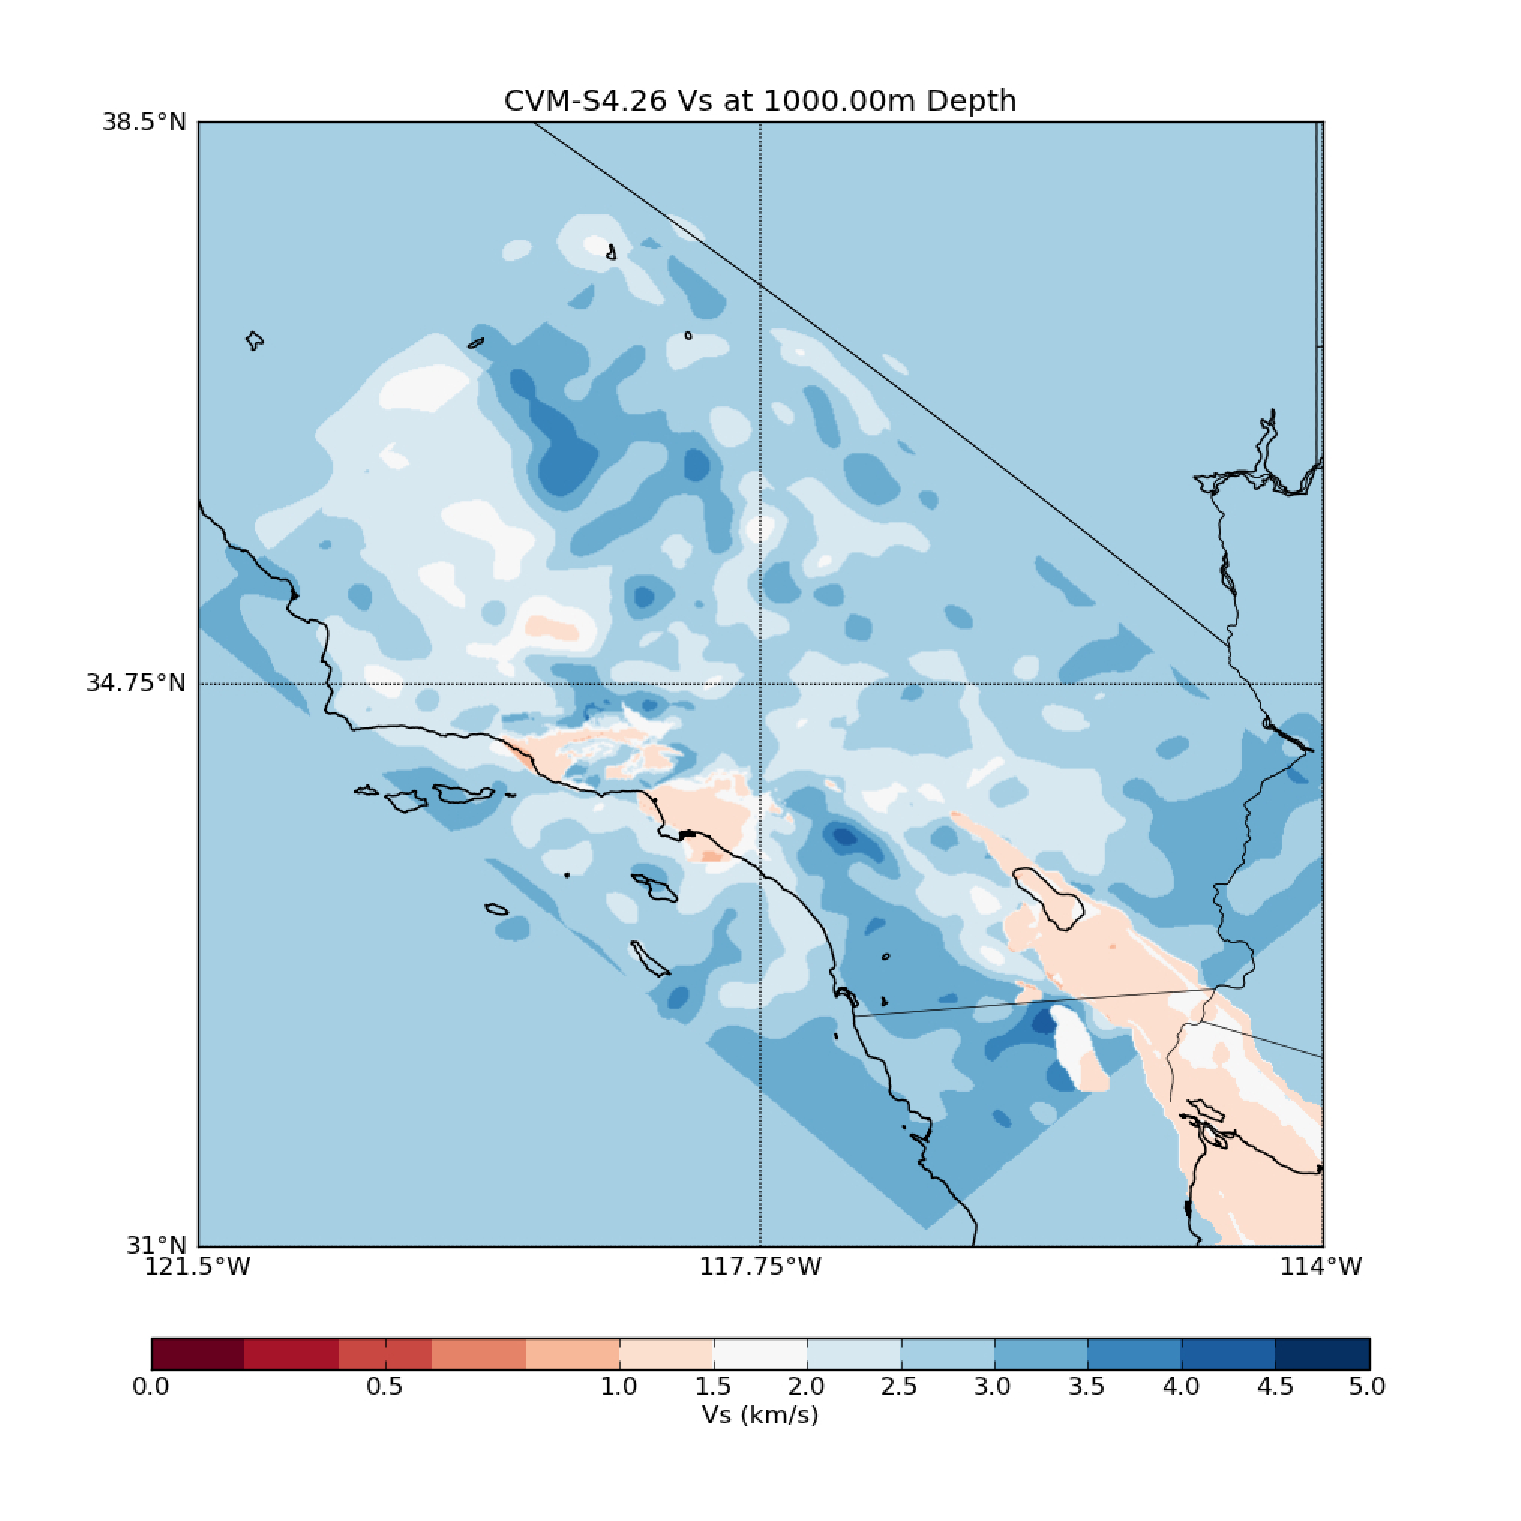
\includegraphics
                [width=0.5\textwidth]
                {figures/pdf/cvms426}

\textcolor{blue}{The map above was generated using the following inputs. User-entered text is denoted in red.}

\begin{lstlisting}[
        frame=none,
        basewidth={0.45em,0.4em},
        basicstyle=\ttfamily\footnotesize,breaklines=true,
        linewidth=0.98\columnwidth,xleftmargin=0.065\columnwidth,
        numbers=left,numberblanklines=true,numberstyle=\scriptsize\color{mylistingnclr},style=output]
> ./horizontal_slice.py
> Plot Horizontal Slice - UCVM 14.3.0
>
> This utility helps you plot a horizontal slice across the earth for one of the CVMs
> that you installed with UCVM.
>
> In order to create the plot, you must first specify the region.
>
> Please enter the bottom-left longitude from which the plot should start: @-121.5@
> Next, enter the bottom-left latitude from which the plot should start: @31@
> Enter the top-right longitude where the plot should end: @-114@
> Enter the top-right latitude where the plot should end: @38.5@
> Which grid spacing (in decimal degree units) would you like (usually, this is 0.01): @0.01@
>
> Please enter the depth, in meters, at which you would like this plot: @1000@
>
> What would you like to plot (either vp, vs, rho, or poisson): @vs@
>
> From which CVM would you like this data to come:
>	1) CVM-S4
>	2) CVM-H 11.9.1
>	3) CVM-H 11.9.1 No GTL
>	4) CVM-S4.26
>	5) 1D
>	6) Broadband Whittier Narrows 1D Model
>	7) 1D w/ Vs30 GTL
>
> Select the CVM: @4@
>
> Finally, would you like a descritized or smooth color scale
> (enter 'd' for discrete, 's' for smooth): @d@
>
> Retrieving data. Please wait...
> Data retrieved successfully.
>
> Would you like to:
>	1) Save the data
>	2) Generate a plot
>
> Select one: @2@
\end{lstlisting}

\textcolor{blue}{All of the plotting scripts bundled with UCVM work in a very similar manner. Launching the script will ask a series of questions asking the user to define the region for the plot, the material property ($V_p$, $V_s$, or $\rho$) to plot, the model from which the data should come, and whether or not to save the data to an ASCII text file or display a graphical PNG image.} 
